\let\negmedspace\undefined
\let\negthickspace\undefined
\documentclass[journal]{IEEEtran}
\usepackage[a5paper, margin=10mm, onecolumn]{geometry}
%\usepackage{lmodern} % Ensure lmodern is loaded for pdflatex
\usepackage{tfrupee} % Include tfrupee package

\setlength{\headheight}{1cm} % Set the height of the header box
\setlength{\headsep}{0mm}     % Set the distance between the header box and the top of the text

\usepackage{gvv-book}
\usepackage{gvv}
\usepackage{cite}
\usepackage{amsmath,amssymb,amsfonts,amsthm}
\usepackage{algorithmic}
\usepackage{graphicx}
\usepackage{textcomp}
\usepackage{xcolor}
\usepackage{txfonts}
\usepackage{listings}
\usepackage{enumitem}
\usepackage{mathtools}
\usepackage{gensymb}
\usepackage{comment}
\usepackage[breaklinks=true]{hyperref}
\usepackage{tkz-euclide} 
\usepackage{listings}
% \usepackage{gvv}                                        
\def\inputGnumericTable{}                                 
\usepackage[latin1]{inputenc}                                
\usepackage{color}                                            
\usepackage{array}                                            
\usepackage{longtable}                                       
\usepackage{calc}                                             
\usepackage{multirow}                                         
\usepackage{hhline}                                           
\usepackage{ifthen}                                           
\usepackage{lscape}
\begin{document}

\bibliographystyle{IEEEtran}
\vspace{3cm}

\title{2.4.23}
\author{EE25btech11028 - J.Navya sri}
% \maketitle
% \newpage
% \bigskip
{\let\newpage\relax\maketitle}




\textbf{Question:}\\
Do the points \( (3, 2) \), \( (-2, -3) \), and \( (2, 3) \) form a triangle? If so, name the type of triangle formed.


\vspace{0.5cm}
\textbf{Solution:}

Given points,

\begin{equation}
A=\myvec{3\\2}, \quad 
B=\myvec{-2\\-3}, \quad 
C=\myvec{2\\3}
\end{equation}

\subsection*{1. Collinearity check (using rank)}

Form the matrix:
\begin{equation}
M=\myvec{
3 & 2 & 1\\
-2 & -3 & 1\\
2 & 3 & 1
}
\end{equation}

Apply row operations:
\begin{equation}
R_2 \leftarrow R_2+2R_1,\quad R_3 \leftarrow 3R_3-2R_1
\;\;\Rightarrow\;\;
\myvec{
3 & 2 & 1\\
4 & 1 & 3\\
0 & 5 & 1
}
\end{equation}

\begin{equation}
R_2 \leftarrow 3R_2-4R_1
\;\;\Rightarrow\;\;
\myvec{
3 & 2 & 1\\
0 & -5 & 5\\
0 & 5 & 1
}
\end{equation}

\begin{equation}
R_3 \leftarrow R_3+R_2
\;\;\Rightarrow\;\;
\myvec{
3 & 2 & 1\\
0 & -5 & 5\\
0 & 0 & 6
}
\end{equation}

Since all three rows are nonzero:
\begin{equation}
\operatorname{rank}(M)=3
\end{equation}

\[
\Rightarrow \text{Points are not collinear, so they form a triangle.}
\]

\subsection*{2. Right-angle check}

\begin{equation}
\overrightarrow{AB}=B-A=\myvec{-5\\-5}, \quad 
\overrightarrow{AC}=C-A=\myvec{-1\\1}
\end{equation}

\begin{equation}
\overrightarrow{AB}\cdot \overrightarrow{AC} = (-5)(-1)+(-5)(1)=0
\end{equation}

\[
\Rightarrow \overrightarrow{AB}\perp \overrightarrow{AC}
\]

So, the triangle is right-angled at
\begin{equation}
A=\myvec{3\\2}
\end{equation}

\subsection*{3. Final Answer}

\begin{equation}
\text{The given points form a triangle (rank = 3).}
\end{equation}

\begin{equation}
\text{The triangle is right-angled at } A=\myvec{3\\2}.
\end{equation}

\textbf{Graphical Representation:}

\begin{center}
\begin{tikzpicture}[scale=0.8]
    % Draw axes
    \draw[->] (-5,0) -- (5,0) node[right] {x};
    \draw[->] (0,-5) -- (0,5) node[above] {y};

    % Grid (optional)
    \draw[step=1cm,gray!30,very thin] (-5,-5) grid (5,5);

    % Points
    \coordinate (A) at (3,2);
    \coordinate (B) at (-2,-3);
    \coordinate (C) at (2,3);

    % Draw triangle
    \draw[thick, blue] (A) -- (B) -- (C) -- cycle;

    % Draw and label points
    \filldraw[black] (A) circle (2pt) node[anchor=west] {A(3,2)};
    \filldraw[black] (B) circle (2pt) node[anchor=east] {B(-2,-3)};
    \filldraw[black] (C) circle (2pt) node[anchor=west] {C(2,3)};
    \end{tikzpicture}
    
        % Add "Fig. 0" text below the figure
    \vspace{0.5cm} % space between figure and text
    \textbf{Fig. 0}

\end{center}

\end{document}


